% Chapter 1 - Estado del Arte

\chapter{Estado del Arte} % Chapter title

\label{ch:estado_arte} % For referencing the chapter elsewhere, use \autoref{ch:introduction} 

%----------------------------------------------------------------------------------------

% ### Introducción de capitulo

A continuación se introducirán las distintas soluciones que conforman el estado del arte actual en cuanto a técnicas que permitan desarrollar aplicaciones con soporte de interacciones multimodales.

Por interacciones multimodales, se hace referencia a todas aquellas interacciones, tanto para con el mundo físico real como para el virtual a través de los diferentes \emph{modos}; cada uno de estos modos esta ``asociado'' a los sentidos del ser humano, de acuerdo a \citet{Bourguet2003}. Se busca, de esta forma, eliminar o disminuir barreras en la comunicación hombre-máquina/aplicación, \eg eliminando o dando una alternativa al uso del clásico teclado/ratón, eligiendo favorecer a nuevas capacidades de interacción naturales.
Cuando se permite operar con mas de uno de estos \emph{modos} en simultaneo, estamos frente a interacciones multimodales.

En este capitulo se analizarán diferentes soluciones, la forma en que se brindan estas soluciones varía según cada trabajo, algunas optan por utilizar un formato tipo framework, es decir como una herramienta de software que puede ser usada para crear otras aplicaciones; otras por una plataforma brindando una solución mas general ó incluso como un servicio web. Para identificar mejor las diferentes soluciones se ha decidido presentar las mismas organizadas de acuerdo al formato (\ie, plataforma, framework, etc.) o al contexto (\ie, educativo, uso general, entre otros). 
Luego se analizan los problemas comunes que pueden padecer estos trabajos y se compara con las estrategias seleccionadas en la solución propuesta. 
Al finalizar el capitulo se encuentra un cuadro que resume las distintas publicaciones mencionadas.


\section{Trabajos Relacionados} \label{sec:related_work} %Detalle de trabajos

\subsection{Clasificación según el Formato}

%tipo: framework - ambito de la solucion: "general" Kenneth et al.
%Introduction to a Framework for Multi-modal and Tangible Interaction
En el trabajo de \citet{lo2010introduction}, se propone un framework de uso general para añadir nuevas modalidades al ámbito de prácticamente cualquier aplicación. Para lograr esto, el framework propuesto, permite controlar una interfaz de acceso a nuevos dispositivos al sistema, estos nuevos dispositivos son los que añaden las nuevas modalidades. Las pruebas que han realizado incluyen hardware como el Wiimote e iPhone. Las modalidades que han sido integradas al framework son: gestual (utilizando las manos), háptica y reconocimiento de voz. A través de una arquitectura de tres capas, las señales producidas por los dispositivos son transformadas en comandos que actúan sobre las aplicaciones.

En un principio este framework esta orientado a disminuir las barreras en la inserción de nuevas modalidades en un sistema previamente desarrollado. 

La solución que se propone en éste trabajo, encuentra similitudes con el acercamiento de \citet{lo2010introduction}, aunque el trabajo aquí propuesto se enfoca directamente en el desarrollo integral de aplicaciones web. Además, si bien existen similitudes arquitectónicas entre las soluciones, como puede ser la separación en capas, dando independencia al ingeniero de modalidad para trabajar con el lenguaje necesario y aun así poder conectarse al framework; en este trabajo se han tomado decisiones novedosas que no se han visto en otros trabajos similares, como la separación y distribución de los componentes de fisión y fusión. En la parte dos se introducen todos los detalles arquitectónicos propios de la plataforma propuesta.


%tipo: framework - ambito de la solucion: aplicaciones moviles
%Multimodal Framework for Mobile Interaction
En el caso de \citet{cutugno2012multimodal}, introducen también un framework que permite añadir interacciones multimodales en dispositivos móviles. La importancia de tener en cuenta estos aparatos se basa en su popularidad y en sus capacidades, muchos cuentan con pantallas sensibles al tacto, cámaras, micrófonos, parlantes y un conjunto de sensores. Es decir, mecanismos que permiten abrir nuevos canales de comunicación con el usuario a través de una herramienta portátil. Otra característica importante, es que en el trabajo de \citet{cutugno2012multimodal}, siguen los lineamientos de la W3C \citep{w3c:mmiframework} \citep{w3c:mmiarch} para producir un framework compatible a estas disposiciones. Las aplicaciones que utilicen este framework podrán recibir notificaciones generadas por un reconocedor de modalidad, es decir existe una vía de comunicación multimodal (entrada). Además, señalan que los desarrolladores pueden indicar a cual evento multimodal suscribirse a través de la generación de un documento XML especifico. Con el uso de este archivo el servidor puede conocer a qué componente de la aplicación cliente alertar cuando ocurre determinado evento multimodal, entre otras funciones; para efectivizar esta comunicación los autores proponen un conjunto de etiquetas basado en SMUIML \citep{dumas2008prototyping}. Otra característica de este trabajo es el uso de NFAs (\emph{Nondeterministic Finite Automaton}) para generar los distintos escenarios posibles de interacción. 

De esta manera el framework genera una aplicación que en el \emph{Interaction Manager} funciona como una maquina de estados. 

El framework es validado a través del desarrollo de una aplicación \emph{Android} que hace uso de GMaps para resolver consultas sobre el transporte público que pueden ser emitidas mediante el uso de gestos táctiles y voz.

El uso de NFA's y de un metalenguaje para representar componentes, son características propias de este trabajo que no se encuentran en la solución propuesta. Se considero como añadir excesiva complejidad, introducir una máquina de estados en el núcleo del \emph{Interaction Manager} de forma tan temprana, cuando lo que se estaba desarrollando era un sistema novedoso, aunque no se descarta una estrategia así para futuras versiones mas estables. Respecto a la decisión de no brindar una representación basada en un metalenguaje, la razón se basa en que esta plataforma no se apoya en un servidor, corre íntegramente en clientes, distribuida; utilizando el servicio de mensajería provisto, el cual se encarga de mantener y distinguir a los diferentes clientes.

%tipo: plataforma - ambito de la solucion: "general"
% i*Chameleon: A Platform for Developing Multimodal Application with Comprehensive Development Cycle
A diferencia de los trabajos anteriores, \citet*{lo2013chameleon} consideran, no solo la construcción de un framework, sino también los aspectos de infraestructura necesarios para interconectar los distintos componentes de la solución, de esta manera se introduce una \textsf{plataforma} para el desarrollo de aplicaciones que soportan interacciones multimodales, la misma es denominada \emph{i*Chameleon}. Proponen un ciclo de desarrollo con una clara división de tareas entre los diferentes responsables de una aplicación multimodal, usando un framework que sigue el patrón MVC. 

De esta forma, los ingenieros de dispositivos son los responsables de integrar nuevos artefactos a la plataforma, según Lo et al. esta etapa corresponde al desarrollo de ``vistas''; luego los diseñadores de modalidades se encargan de crear la modalidad a utilizar, la misma puede estar compuesta por uno o mas componentes encargados de analizar los datos de la modalidad. Estos componentes son los ``modelos'' dentro del framework. Luego de que la modalidad ha sido diseñada es momento de implementar el nivel de fusión de la misma. Los desarrolladores son los encargados de esta tarea que se corresponde al componente ``controlador'' del framework. Finalmente, los diseñadores de interacción son los encargados de generar la aplicación; para conseguir esto \emph{i*Chameleon} brinda una interfaz de alto nivel, lograda gracias a la separación de responsabilidades antes mencionada, de esta forma no es necesario tener conocimientos de programación para llevar a cabo esta etapa (diseño de interacción).

En \emph{i*Chameleon} se destaca claramente la separación de responsabilidades de un equipo de desarrollo multimodal, esto lo consiguen a través del desarrollo y uso de un framework modular. Este aspecto es similar a lo que se propone en el presente trabajo y mas aun, se busco mantener esta separación de tareas y roles.

\marginpar{El ciclo de desarrollo profesional en aplicaciones multimodales es multidisciplinario. El mismo puede estar compuesto por: desarrolladores, ingenieros de modalidad, psicólogos y desarrolladores de interacción; entre las profesiones destacadas.}

\subsection{Clasificación según el Dominio}

%tipo: framework - ambito de la solucion: smart environment
%An innovative framework to support multimodal interaction with Smart environments.
\citet{gabbanini2012innovative} introducen un framework donde el foco esta puesto en los entornos inteligentes. En dichos entornos, la presencia de múltiples dispositivos que interactúan de alguna manera con el usuario es algo común, por lo tanto contar con una estrategia para aprovechar estos recursos de forma organizada es importante según establecen los autores. Una de las características de este trabajo son los principios que establecen para el diseño de interacciones multimodales,  se fijan tres, son: 
(1) no establecer relaciones de dependencia entre modalidades, (2) respetar y explotar las características de cada modalidad y (3) modelar criteriosamente las actividades que podrá desarrollar el usuario. Dentro del framework manipulan una máquina de estados, la misma permite modelar las transiciones de una modalidad. Cada estado representa una forma controlada de respuesta a un evento. Un evento puede ser generado por el uso de una modalidad. Al igual que en el caso de \emph{i*Chameleon} los autores mencionan la necesidad de no perder de vista el rasgo integrador en cuanto a las distintos tipos de profesionales (desde programadores e ingenieros hasta psicólogos y desarrolladores de interacción), que son necesarios para el desarrollo de una correcta aplicación multimodal.

Así, \citet{gabbanini2012innovative} desarrollan una aplicación multimodal particular que hace uso del canal de voz y auditivo.


%tipo: framework/environment - ambito de la solucion: educativo (e-learning)
%e-Learning Environment with Multimodal Interaction
Un punto de vista diferente que pone las características de una aplicación multimodal como una necesidad es expuesto por da Silva \& da Rocha \citep{da2013learning}. El contexto de las aplicaciones analizadas es el ámbito educativo. Particularmente aplicaciones web como \emph{moodle}, \emph{sakai} o la brasileña \emph{teleduc} fueron tenidas en cuenta en el trabajo. Los autores plantean como hipótesis que añadir interacciones multimodales a estas aplicaciones mejorará no sólo la usabilidad sino también la accesibilidad de las mismas. 

Para probarlo construyen un ambiente web educativo, extendiendo \emph{Ae e-Learning environment}, para que tenga soporte a interacciones multimodales; a través del uso de este framework los autores esperan obtener mediciones concretas que validen su teoría. 
Utilizan las modalidades gestuales y hápticas (táctil) como canales de entrada al sistema que hacen juego con determinados componentes del entorno educativo como son el \emph{Weblog} y el \emph{Whiteboard}.

%tipo: framework - ambito de la solucion: general movil
%A Framework for the Development of Distributed Interactive Applications
Finalmente, cabe destacar el enfoque transversal que hacen las técnicas multi-dispositivo, en particular el desarrollo de interfaces de usuario distribuidas. Si bien esta temática no tiene como objetivo el soporte a múltiples modalidades, el efecto de expandir el contenido a otros dispositivos tales como tablets o smartphones hace posible que dichos contenidos puedan ser accedidos a través de otras modalidades, como pueden ser gestos táctiles. Por lo tanto es interesante tener en cuenta el desafío técnico que se realiza en esta área.
En particular se analiza el trabajo de \citet{frosini2013framework}, donde exponen tanto un framework como aspectos detallados de la arquitectura de la solución. 

Uno de los puntos destacados es el estilo distribuido de la solución, el framework se divide en dos partes, una de las cuales reside en los dispositivos clientes (\emph{client side}); la otra puede estar en un servidor (\emph{engine side}). De esta forma, los distintos dispositivos, que pueden contar con capacidades diferentes de interacción, pueden procesar no solo la lógica de la aplicación sino también señales del framework (\nolinebreak{\emph{engine side}}). Así pueden distinguirse diferentes responsabilidades, los dispositivos \emph{client side}, pueden decidir como actuar y qué eventos o notificaciones ``escuchar'' del \emph{engine side}; también se destaca la necesidad de un sistema de mensajería entre los distintos componentes del sistema como un aspecto importante. Estas características arquitectónicas encuentran similitudes con las de la solución aquí presentada, en aspectos tales como, distribuir parte de la lógica del framework en los clientes o utilizar un sistema de mensajería y señalización para comunicarse con los clientes.

\section{Aspectos de Diseño}
Continuando con la clasificación propuesta, se analizarán primero los desafíos que deben superar las soluciones desde el punto de vista del formato. Luego se considerarán los trabajos de acuerdo a la forma de instanciar y utilizar el framework en la práctica.

Desde el punto de vista del formato, un requisito importante es la modularidad del sistema. Esto converge de diferentes fuentes, como \citet{dumas2009multimodal} o el grupo de trabajo de la W3C respecto a arquitecturas multimodales \citep{w3c:mmiarch}, donde se distinguen al menos cuatro módulos que permiten una clara separación de responsabilidades, estos son: 
\begin{itemize}
\item
Componentes de modalidad de entrada y salida (\emph{Input \& Output modalities}),también conocidos como reconocedores y sintetizadores de modalidad, a veces pueden ser un único componente.
\item
Comité de integración (\emph{Integration Committee}), el encargado de mantener la lógica de coordinación de las diferentes modalidades. Aquí se encuentran dos módulos importantes que serán especificados mas adelante; son los componentes de fusión y de fisión.
\item
Administrador de dialogo (\emph{Dialog Manager}), a veces considerado parte del comité de integración, este componente es el encargado de manejar la comunicación entre aplicación y los componentes de fusión y fisión.
\item
Aplicación (o también \emph{Runtime Framework}), el sector de nuestro sistema donde comenzaremos a instanciar las diferentes partes que componen el dominio del problema de la aplicación particular. 
\end{itemize}
Una clara separación de los componentes posibilita el desarrollo en paralelo de los mismos así como beneficia la escalabilidad del sistema en general. Mas información sobre la implementación de la plataforma se verá en la segunda parte (capítulos: \ref{ch:infra} y \ref{ch:enlace}).

Tanto en \emph{MIF}\citep{lo2010introduction} como en \emph{i*Chameleon}\citep{lo2013chameleon} se presentan soluciones modulares, por ejemplo en el gráfico ~\ref{fig:mfi_action}, se muestran los diferentes módulos de MFI en acción. 

Particularmente, \emph{i*Chameleon} presenta una arquitectura que se adapta casi directamente a la referenciada anteriormente. En \emph{MIF}, los autores eligen otro acercamiento, en un framework de tres capas donde ponen énfasis en la integración de nuevas modalidades a aplicaciones existentes. 

% FIGURA DE MODULOS MFI
\begin{center}
  \begin{figure}[h]
    \centering

    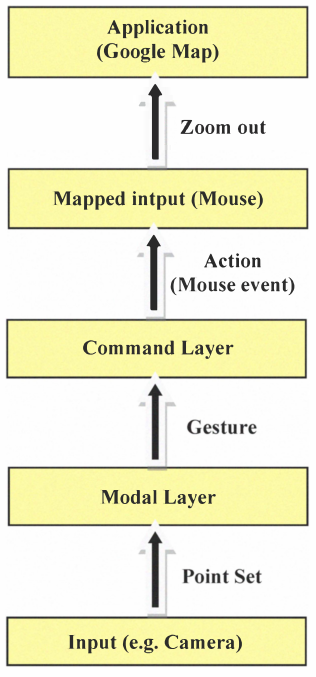
\includegraphics[scale=0.5]{gfx/mfi_modules_action}
    \caption{Módulos de MFI en acción.}
    \label{fig:mfi_action}
  \end{figure}
\end{center}

Otro factor de diseño importante es la capacidad de añadir nuevas modalidades. Es decir, el soporte que se brinda al desarrollador, desde el framework o plataforma, para agregar una nueva modalidad al sistema. En muchos casos, solo se considera un subconjunto de tecnologías particulares, en lugar de un subconjunto de modalidades en general. Por ejemplo, no es lo mismo un framework que permite el desarrollo de aplicaciones que hacen uso del \textsf{Novint Falcon}\footnote{Falcon de la compañía Novint, es un dispositivo que permite generar feedback háptico mediante la utilización de un sistema de servo-motores especialmente diseñado. Para mas información sobre el producto pueden visitar el sitio de  \href{http://www.novint.com/index.php/novintfalcon}{Novint}. Para conocer mas sobre la modalidad háptica pueden dirigirse al apéndice \ref{ch:mod_air}.} exclusivamente, que otro que posibilita el desarrollo de aplicaciones que hagan uso de la modalidad háptica en general(\eg, \emph{MIF}). En este punto ambos trabajos presentan buenas soluciones. En particular, en \emph{i*Chameleon} se distingue una etapa del ciclo de desarrollo, la de integración de driver de dispositivo (\emph{Device Driver Integration}), donde los ingenieros de dispositivos pueden desarrollar los módulos necesarios para conectarlos al sistema, los mismos incluso pueden ser re-utilizados, lo que avala técnicas como DRY y minimiza el grado de error.
\linebreak
Siguiendo con la división planteada, se revisan los aspectos de diseño en trabajos donde la atención está puesta en frameworks que brindan soluciones a problemas específicos  \ie, entornos educativos, ambientes inteligentes, dispositivos móviles, etc.
Entonces los siguientes aspectos serán de interés: re-usabilidad de componentes multimodales, extensibilidad del framework, orientado a ciclo de desarrollo y facilidad de uso. Estos, entre otros aspectos, son tratados por \citet{dumas2009multimodal}.

Aquí se destaca el enfoque de \citet{cutugno2012multimodal}, en dicho trabajo descentralizan el framework consiguiendo distribuir la lógica entre servidor y clientes \ie, estos últimos pueden procesar el mecanismo de fisión. Esta separación es lograda a través del uso de un archivo XML de configuración. Por medio de este archivo el desarrollador puede:
\begin{itemize}
\item
Especificar los eventos que pueden generar un cambio de estado.
\item
Indicar los comandos que el usuario puede disparar del lado cliente.
\item
Indicar cómo el usuario puede activar estos comandos a través de las modalidades.
\end{itemize}
De esta forma, este archivo representa una abstracción, que le permite al desarrollador indicar cuales comandos podrán ser lanzados y a través de que acciones multimodales, todo esto a través de claras etiquetas XML. Así el sistema brinda facilidad de uso y una posibilidad de re-usabilidad de componentes multimodales, la cual depende de la configuración XML del framework y la posibilidad de compartirla entre otras instancias del mismo. Si bien el trabajo de \citet{da2013learning} es un trabajo en progreso, tiene gran potencial para demostrar extensibilidad del framework multimodal y facilidad de uso, ya que estas plataformas de educación online son utilizadas en diferentes ámbitos por un gran conjunto de usuarios finales y no solo desarrolladores experimentados.
Finalmente, es notable el trabajo de \citet*{lo2013chameleon} ya que además de considerar a la plataforma necesaria junto al framework, los autores incluyen diversos aspectos, como técnicas que posibilitan re-utilizar interacciones multimodales entre distintas aplicaciones. También presentan un caso de desarrollo completo de una aplicación, haciendo énfasis en la clara separación de responsabilidades que brinda su herramienta, la cual es conseguida gracias al alto grado de modularización del framework; estos distintos componentes pueden asociarse claramente a los distintos roles involucrados en el desarrollo integral de una aplicación multimodal. De esta manera, es posible dividir exitosamente el trabajo entre los distintos profesionales que intervienen en el desarrollo, estos son: ingenieros de dispositivo, diseñadores de modalidad, programadores y diseñadores de interacción.

\subsection{Sobre la Plataforma Propuesta}
Teniendo en cuenta estos factores de diseño, la estrategia presentada en este trabajo presenta una arquitectura de componentes, similar a la propuesta por la W3C, la cual tendrá como objetivos definir claramente responsabilidades y facilitar tanto la extension de la plataforma como así también aspectos de escalabilidad de la misma. En cuanto al soporte para añadir nuevas modalidades, se aprovecha la separación de responsabilidades antes mencionada, introduciendo una etapa similar a la de integración de dispositivo de \emph{i*Chameleon} con el agregado de un protocolo de comunicación que permita facilitar la inserción de nuevo hardware.
También se tendrá en cuenta, lograr una plataforma fácil de usar por los desarrolladores de aplicaciones web. La posibilidad de conectar nuevas modalidades estará dada por los módulos desarrollados por los ingenieros de modalidades; como el desarrollo de los mismos no esta atado a un lenguaje en particular, la posibilidad de compartirlos para re-utilizarlos no será tan directa, aunque si se gana en flexibilidad. Por otra parte, se considerará brindar una clara separación en componentes, de los cuales se puedan etiquetar claramente las responsabilidades. Con respecto a la capacidad de extender la plataforma, en principio se plantea como para ser extendida ``a los extremos'', es decir que no solo se contempla el crecimiento a través de la conexión de nuevas modalidades sino también desde el lado cliente, por medio de lo que pueden ser diferentes módulos que agreguen capacidades ''extra'' en la interacción con la aplicación y con las nuevas señales que esta recibe (producidas por las modalidades).

\section{Comparación del Escenario Actual}
La tabla ~\ref{tab:estado_arte_tabla} compara algunas de las soluciones tratadas en este capitulo. Se considera: si se soporta un canal de entrada y salida para la modalidad, se aclara si es de propósito general o no y cual es el grado de soporte al desarrollo de aplicaciones web en particular.

%\begin{landscape}
\begin{sidewaystable}[p]
%  \begin{table}
%	  \begin{tabularx}{630pt}{p{4.8cm}|p{2.2cm}|p{2.2cm}|p{3.5cm}|p{3.4cm}|p{3.6cm}}
%	  \begin{tabularx}{600pt}{p{4.6cm}|p{2.2cm}|p{2.2cm}|p{2.4cm}|p{3.2cm}|p{3.6cm}}
 	  \begin{tabularx}{565pt}{p{4.4cm}|p{2.2cm}|p{2.2cm}|p{2cm}|p{3.2cm}|p{3.6cm}}
      \toprule[2pt]
	    \tableheadline{Trabajos - Propiedad} & 
	    \multicolumn{1}{p{2.2cm}}{Modalidad: Entrada} & 
	    \multicolumn{1}{p{2.2cm}}{Modalidad: Salida} & 
	    \multicolumn{1}{p{2cm}}{Ámbito de la solución} &
	    \multicolumn{1}{p{3.2cm}}{Orientado a ciclo de desarrollo MMI} & 
	    \multicolumn{1}{p{3.6cm}}{Soporte al desarrollo de aplicaciones web} \\ 
	    \midrule
	    Introduction to a Framework for Multi-modal and Tangible Interaction &
	    Si &
	    Limitada &
	    General &
	    No \footnote{Los casos negativos o de ausencia de alguna propiedad, se deben a no estar explícitamente indicados en los trabajos, todas las soluciones analizadas presentan buenas practicas de desarrollo de software. \label{fn:review_note_no}}&
	    Medio \\
	    \midrule
	    i*Chameleon &
	    Si & 
	    Si & 
	    General & 
	    Si & 
	    Medio \\
 	    \midrule
 	    An innovative framework to support multimodal interaction with Smart environments. &
      Si &
      Limitada &
      Smart Environments &
      Parcial \footnote{Arq. en componentes, clara separación de los mismos pero no hay aclaración en el trabajo sobre este aspecto. \label{fn:review_note_parcial}} &
      Bajo \\
 	    \midrule
   	  e-Learning Environment with Multimodal Interaction &
   	  Si & 
   	  No &
   	  Plataformas Educativas, accesibilidad &
   	  No \footref{fn:review_note_no} &
   	  Medio \\
 	    \midrule
  	  Multimodal Framework for Mobile Interaction &
  	  Si &
  	  No &
  	  Dispositivos Móviles &
  	  Parcial \footref{fn:review_note_parcial} & % 
  	  Medio \\
 	    \midrule
 	    A Framework for the Development of Distributed Interactive Applications &
 	    Posible &
 	    Posible &
 	    UI Multi-dispositivo &
 	    No \footref{fn:review_note_no}&
 	    Bajo \\
	    \bottomrule
	  \end{tabularx}
	  \caption{Escenario actual en soporte multimodal para aplicaciones.}
    \label{tab:estado_arte_tabla}
%	\end{table}
%\end{landscape}
\end{sidewaystable}
\pagebreak

\section{Resumen del Capítulo}\label{sec:estado_arte_summary}
Se han analizado seis trabajos que representan la vanguardia en cuanto a tecnologías para el desarrollo de aplicaciones multimodales. Los mismos fueron clasificados de acuerdo al formato y a la especificidad de la solución. Entre los trabajos revisados se encuentra también el análisis de un framework para el desarrollo de aplicaciones multi-dispositivo con interfaces de usuario migratorias; este trabajo se considera como transversal a los otros y puntualmente son de interés las soluciones arquitectónicas que brinda a un problema similar. 

También se destaca la plataforma propuesta por \citet*{lo2013chameleon} como la solución mas completa y de referencia para este trabajo. Luego se analizan algunos aspectos de diseño que deben sortear tecnologías de este estilo. Se analiza: modularidad de la plataforma en relación a arquitecturas conceptuales como la de la W3C \citep{w3c:mmiarch}, facilidad para añadir nuevas modalidades, posibilidad de re-utilizar modalidades, extensibilidad, facilidad de uso para los desarrolladores al menos y soporte para un ciclo de desarrollo. También se exponen las estrategias seleccionadas por la solución aquí propuesta. 

Finalmente se presenta un cuadro que sumariza algunas de las características mas importantes de los trabajos analizados.

% # FIN
%############################################################################